\section{Other Applications}

\subsection*{Mupltiplication of Large Integers}

\begin{frame}
    \frametitle{큰 수의 곱셈}

    \begin{itemize}
        \item<1-> 자리수 마다 다항식의 항이라고 생각
        \item<2-> \(123456789 \rightarrow 9 + 8x + 7x^2 + \cdots + x^8\)
        \item<3-> FFT\,를 이용해 곱하고 받아올림만 잘 처리하면 끝!
        \item<4-> \(\O(n^{\log_2{3}})\)\,인 Karatsuba\,보다 빠르다!
    \end{itemize}

\end{frame}

\subsection*{Multipoint Evaluation in \texorpdfstring{\(\O(n \log^2 n)\)}{O(nlog2n)}}

\begin{frame}
    \frametitle{Multipoint Evaluation}

    \begin{exampleblock}{\href{https://www.acmicpc.net/problem/18354}{18354번: 다항식과 쿼리 2}}
        다항식 \(f(x)\)\,와 점 \(x_i\)\,가 주어질 때 \(f(x_i)\!\!\mod{1,030,307}\)\,을 계산하세요.
    \end{exampleblock}

    \pause

    \begin{itemize}
        \item 앞 문제와 유사해 보이지만 전혀 다름 \pause
        \item \(786,433 = 3 \times 2^{18} + 1\)\,이기 때문에 \(\omega\)\,를 찾아 NTT\,로 해결 가능 \pause
        \item \(1,030,307 = 2 \times 515,153 + 1\)
        \item \(515,153 = 2^4 \times 11 \times 2,927 + 1\) \pause
        \item 잘 안 됨 ...
    \end{itemize}

    \pause

    임의의 점에 대해 \alert{빠르게} 계산하는 방법?
\end{frame}

\begin{frame}
    \begin{theorem}[나머지정리]
        다항식 \(f(x)\)\,를 \(x - x_i\)\,로 나눈 나머지는 \(f(x_i)\)\,이다. 즉,
        \[
            f(x) \equiv f(x_i) \pmod{x - x_i}
        \]
        이다.
    \end{theorem}

    \pause

    \begin{itemize}
        \item Segment Tree\,를 구성 \pause
        \item 구간 \([l, r)\)\,은 \alert{\(P_{l, r}(x)\)}\,를 나타냄
              \[
                  P_{l, r}(x) = (x - x_l)(x - x_{l + 1})\cdots(x - x_{r - 1})
              \]
    \end{itemize}
\end{frame}

\begin{frame}
    \frametitle{Polynomial Tree}

    \begin{center}
        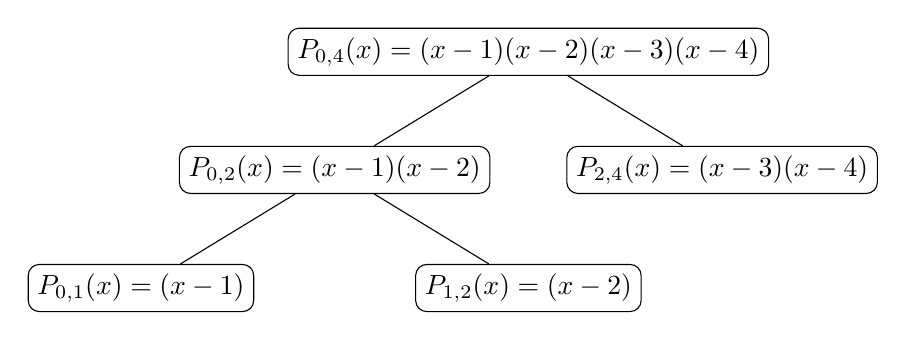
\begin{tikzpicture}[sibling distance=14em,
                every node/.style = {shape=rectangle, rounded corners,
                        draw, align=center
                    }]]
            \node {\(P_{0, 4}(x) = (x - 1)(x - 2)(x - 3)(x - 4)\)}
            child { node {\(P_{0, 2}(x) = (x - 1)(x - 2)\)}
                    child { node {\(P_{0, 1}(x) = (x - 1)\)}}
                    child { node {\(P_{1, 2}(x) = (x - 2)\)}}
                }
            child { node {\(P_{2, 4}(x) = (x - 3)(x - 4)\)}};
        \end{tikzpicture}
    \end{center}

    \pause

    \begin{itemize}
        \item Leaf 노드에서 올라가면서 다항식을 곱하자! \pause
        \item 트리 구성에 들어가는 비용
        \begin{itemize}
            \item 두 subtree\,의 root\,를 곱하는 비용 \(\O(n \log n)\) (FFT)
            \item 왼쪽, 오른쪽 subtree\,는 차수가 절반이므로 각각 \(T\left(\dfrac{n}{2}\right)\) \pause
        \end{itemize}
        \item \(T(n) = \ds 2 T\left(\frac{n}{2}\right) + \O(n \log n) \implies T(n) \in \alert{\O(n\log^2 n)}\)
    \end{itemize}
\end{frame}

\begin{frame}
    \frametitle{Polynomial Tree}
    \begin{center}
        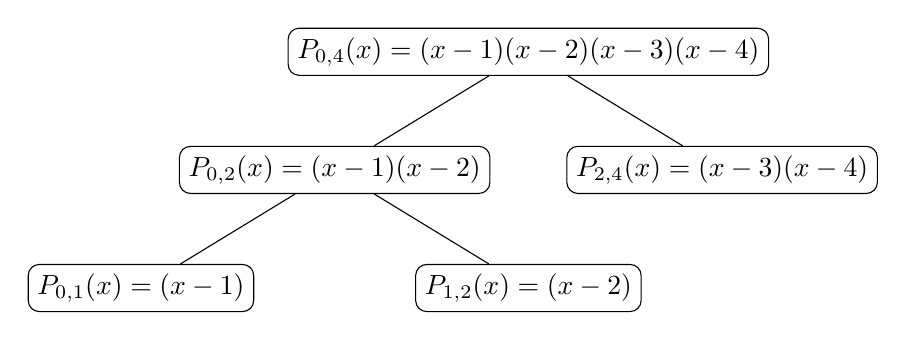
\begin{tikzpicture}[sibling distance=14em,
                every node/.style = {shape=rectangle, rounded corners,
                        draw, align=center
                    }]]
            \node {\(P_{0, 4}(x) = (x - 1)(x - 2)(x - 3)(x - 4)\)}
            child { node {\(P_{0, 2}(x) = (x - 1)(x - 2)\)}
                    child { node {\(P_{0, 1}(x) = (x - 1)\)}}
                    child { node {\(P_{1, 2}(x) = (x - 2)\)}}
                }
            child { node {\(P_{2, 4}(x) = (x - 3)(x - 4)\)}};
        \end{tikzpicture}
    \end{center}

    \begin{itemize}
        \item<1-> Root 노드에서 시작하여 \(f(x) \pmod{P_{l, r}(x)}\) 계산
        \item<2-> 계산 결과를 노드에 저장하고 결과를 subtree\,로 가져가 재귀 호출
        \item<3-> Leaf\,까지 내려오면 \(f(x_i)\)\,가 구해져 있음
    \end{itemize}
\end{frame}

\begin{frame}
    \frametitle{Polynomial Tree}
    \begin{center}
        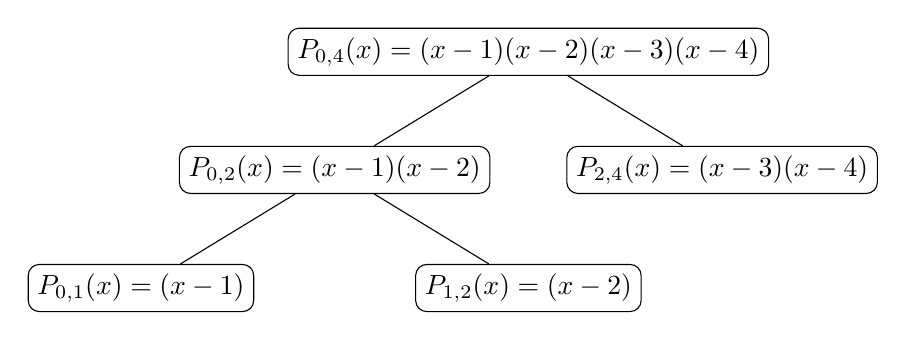
\begin{tikzpicture}[sibling distance=14em,
                every node/.style = {shape=rectangle, rounded corners,
                        draw, align=center
                    }]]
            \node {\(P_{0, 4}(x) = (x - 1)(x - 2)(x - 3)(x - 4)\)}
            child { node {\(P_{0, 2}(x) = (x - 1)(x - 2)\)}
                    child { node {\(P_{0, 1}(x) = (x - 1)\)}}
                    child { node {\(P_{1, 2}(x) = (x - 2)\)}}
                }
            child { node {\(P_{2, 4}(x) = (x - 3)(x - 4)\)}};
        \end{tikzpicture}
    \end{center}

    \begin{itemize}
        \item<1-> 최종 시간 복잡도
        \begin{itemize}
            \item<2-> 현재 노드에서 \(P_{l, r}(x)\)\,로 나누는데 걸린 시간 \(\O(n\log n)\)
            \item<3-> 왼쪽, 오른쪽 subtree\,는 차수가 절반이 되므로 각각 \(T\left(\dfrac{n}{2}\right)\)
        \end{itemize}
        \item<4-> \(T(n) = 2T\left(\dfrac{n}{2}\right) + \O(n\log n) \implies T(n) \in \alert{\O(n \log^2 n)}\)
    \end{itemize}
\end{frame}

